
\subsection{Filtering Techniques}

\subsection{Fast Fourier Volume Registration}

3D phase correlation is CPU and GPU intensive, so in order to reduce complexity we tried to minimize processing in areas which require the most computation time. In out Fourier based volume registration method defined in the previous section, this occurs in the two 3D phase correlations which need to be computed. We describe the method of reduction here; a block diagram for this technique is given in figure \ref{fig:PIPELINE3} WARNING:Given a picture for the sped up version too!. We refer to this method as fast volume registration (FVR) in reference to general volume registration (VR). The speedup begins by computing the 3D DFT of both input volumes and taking the magnitude of these. Rather than directly performing a 3D log-spherical transform and a 3D phase correlation operation on these volumes, we use a novel transform we call a spherical-map transform (details in \ref{SMTransform}).\\

\begin{figure*}[t]
\centering
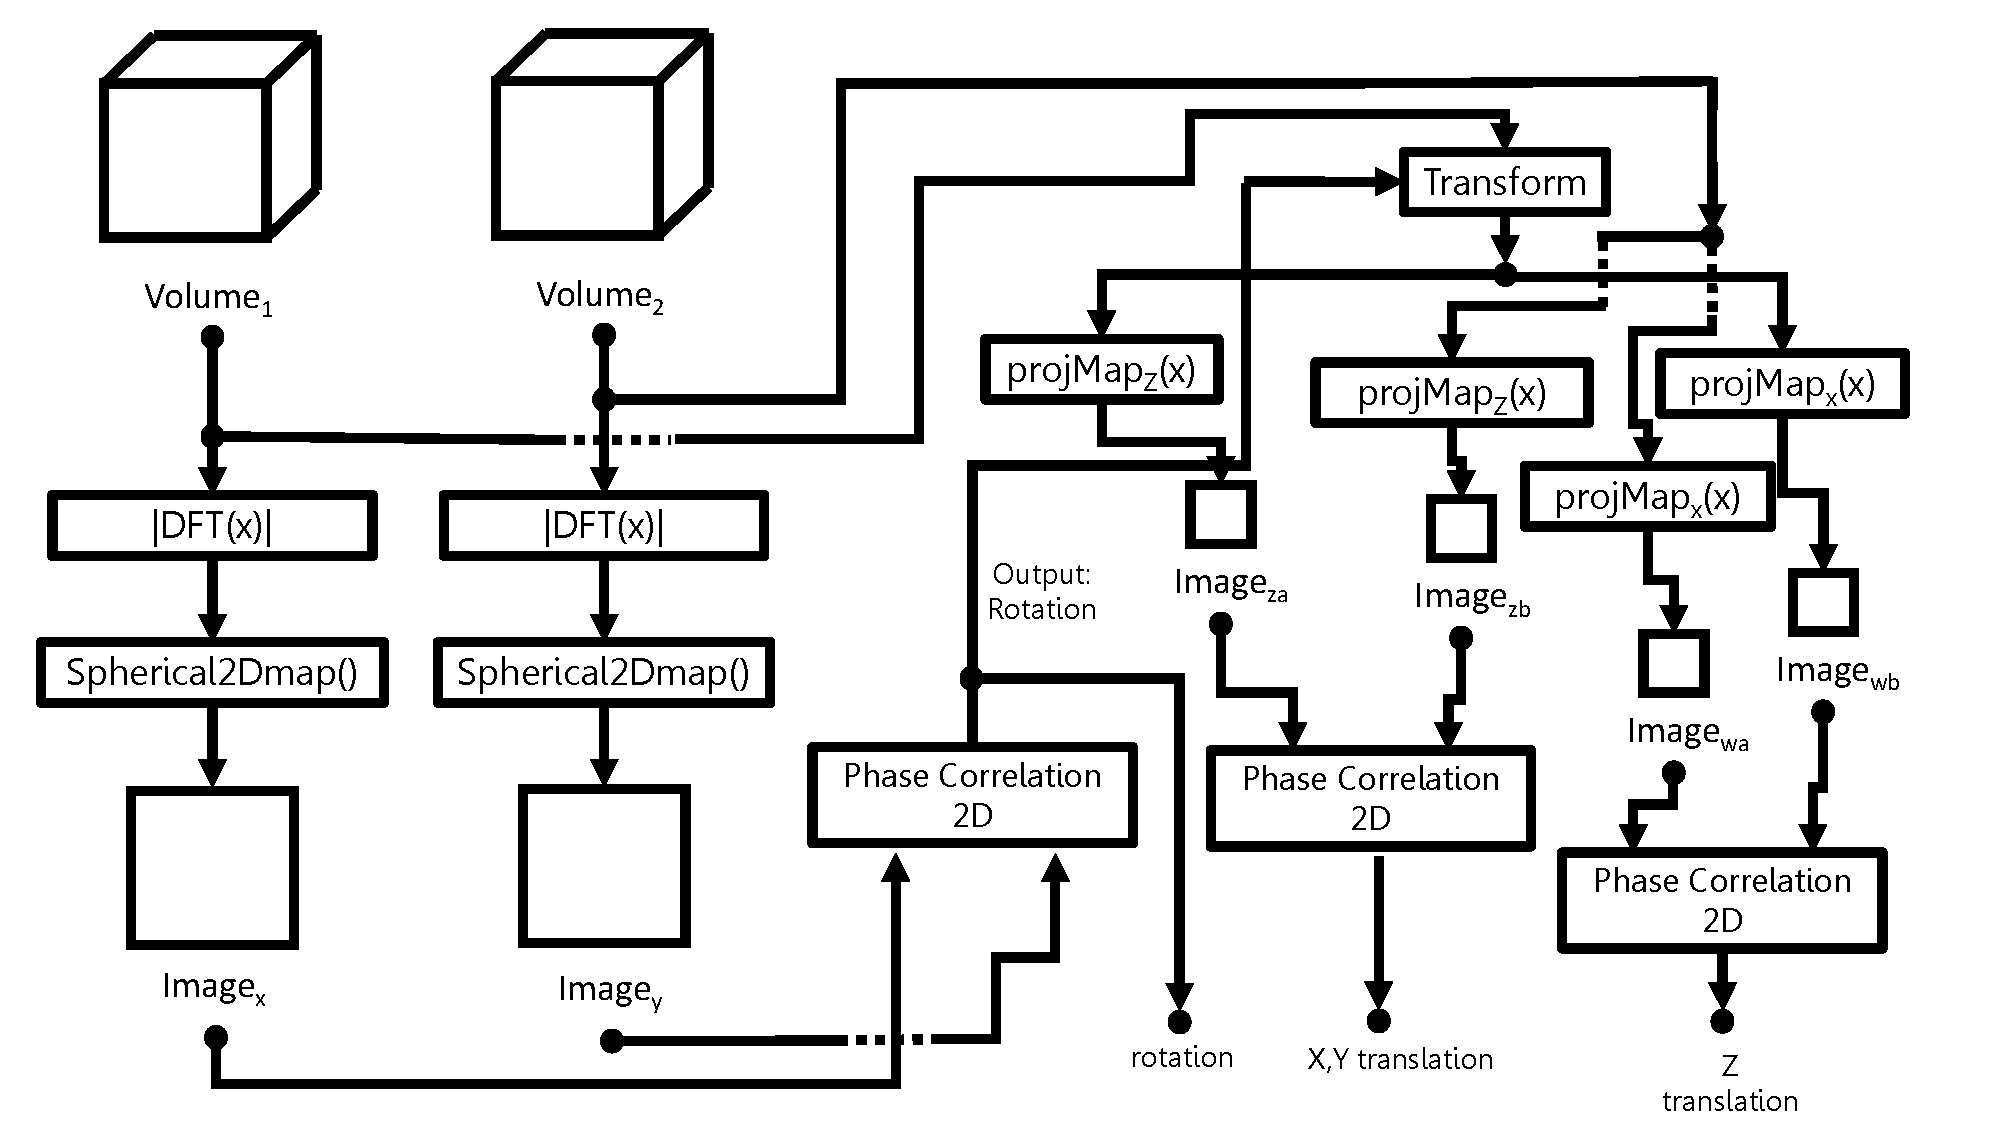
\includegraphics[width=6.0in]{images/ch2/pipeline3}
\caption{System Diagram for Fast Volume Registration}
\label{fig:PIPELINE3}
\end{figure*}

This transform converts rotation into translation whilst simultaneously unfolding the 3D space down to 2-dimensions. After this, a 2D phase correlation that requires significantly less processing compared with the 3D counterpart is used to compute the rotation. Next, having obtained the rotation parameter, the rotation is eliminated from the transformation by rotating the first volume by this parameter. The two volumes are then passed through two orthogonal projection mapping functions. This also converts the volumes to 2D space. We use two transforms for both volumes, one projection along the x-axis, another along the z-axis. Once the x-axis projections of both volumes are complete, we can do another 2D phase correlation to give us the z-translation. The 2D phase correlation of the z-axis projections gives us the x and y axis translations separating the original volumes. The final output of this method gives the rotation and translational shifts between the input volumes. The projections add little complexity to the overall algorithm and since 2D phase correlation operations are used in place of 3D ones, much computation time is reduced.

\subsection{Spherical-map transform}
\label{SMTransform}
The spherical map transform both reduces the 3D volume to a 2D image, and any rotation about the y-axis becomes x-axis translation in the output image. An example of the bunny model and the spherical-map transform of this model is given in figure \ref{fig:smtExample}, the mathematics are defined in equations \ref{eqn:invLPFuncs} and \ref{eqn:smtUpdate}. Given a coordinate in 2D Cartesian space x,y, we compute the ray $[Ray_x Ray_y Ray_z]^T$ from the volume center and sum up the voxel values along the ray (equation \ref{eqn:smtUpdate}). \\


\begin{equation} \label{eqn:invLPFuncs}
\begin{split}
Ray_x(x,y) & = cos\left(\frac{360x}{N}\right)sin\left(\frac{180y}{N}\right)  + \frac{N}{2} \\
Ray_y(y) & = cos\left(\frac{180y}{N}\right) + \frac{N}{2} \\
Ray_z(x,y) & = 	sin\left(\frac{360x}{N}\right)sin\left(\frac{180y}{N}\right) + \frac{N}{2}
\end{split}
\end{equation}

\begin{equation} \label{eqn:smtUpdate}
Im_{x,y} = \sum_{r=1}^{(2^{-1}N)^{1.5}}{Vol(Ray_x(x,y)r, Ray_y(y)r, Ray_z(x,y)r)} 
\end{equation}

This process essentially sums up the values along a given ray defined by scaling spherical coordinates and adding up the values intersecting the ray. The resulting image, maps 3D y-axis rotation to 2D x-axis translation.  \\

\begin{figure*}[t] 
        \centering
        \begin{subfigure}[b]{4.2in}
                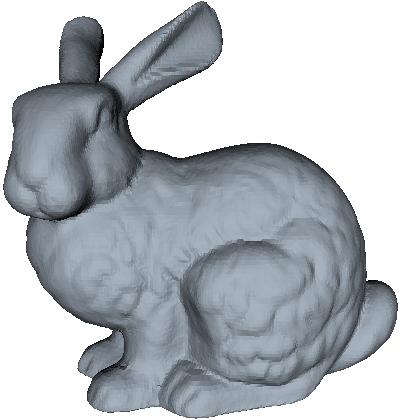
\includegraphics[width=4.2in]{images/ch2/bunny}
                \caption{original}
                \label{fig:bunnyOrig}
        \end{subfigure}
        \begin{subfigure}[b]{4.2in}
                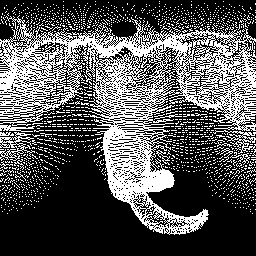
\includegraphics[width=4.2in]{images/ch2/spherical2DMap}
                \caption{transform}
                \label{fig:bunnySPTed}
        \end{subfigure}%
        \caption{The Spherical Map Transform.}
       \label{fig:smtExample}
\end{figure*}


\subsection{Projection-map transform}

The projection map transform is similar to an orthogonal projection of the volume along some given axis. For the projection map transform, given an output image $Im_a$ and an input volume $Vol_a$, each pixel in $Im_a$ is defined mathematically as the summation of values along a particular axis given the image coordinates. The x-axis transform and the z-axis transform are defined in equations \ref{eqn:xPMT} and \ref{eqn:zPMT} respectively. \\

WARNING: add in a picture here

\begin{equation} \label{eqn:xPMT}
Im(z,y) = \sum_{x=0}^{N}{Vol_a(x,y,z)}
\end{equation}

\begin{equation} \label{eqn:zPMT}
Im(x,y) = \sum_{z=0}^{N}{Vol_a(x,y,z)}
\end{equation}

The process defined by equation \ref{eqn:xPMT} maps 3D z-axis translation to 2D x-axis translation, whilst equation \ref{eqn:zPMT} maps 3D x-axis and y-axis translation into 2D x-axis and y-axis translation.


To assess the performance of our method, the size of the volumes being registered is defined as $N^3$ whilst each frame is sampled at a resolution of $W$ $\times$ $H$. The projection process requires $12WH$ operations whilst re-sampling the point cloud requires $2WH$ operations. The Volume Registration process, $VolumeRegister{\theta \varphi t_x t_y t_z}(V_1, V_2)$ consists of 2 $\times$ Hanning windowing processes, 2 $\times$ 3D FFTs, 2 $\times$ volume-logs, 2 $\times$ log-spherical transforms, 2 $\times$ phase correlation processes and 1 $\times$ linear transformation and peak finding. 

The Hanning windowing function requires 26 operations. The 3D FFT has complexity of $3N^3\log{N}$, the log and log-spherical transform functions require 3 and 58 operations per voxel respectively. Multiplying two frequency spectra together and transforming a volume requires 15 and 30 operations per voxel respectively. Finding the peak value requires $2N^3$ operations. The complexity in terms of number of operations for the phase correlation process is given in Eq. \ref{eqn:PCFULLPERFORMANCE} This process requires 2 $\times$ 3D FFTs, 1 $\times$ frequency spectra multiplication, and 1 $\times$ peak finding operation. 
\begin{equation} \label{eqn:PCFULLPERFORMANCE}
6N^3\log{N} + 2N^3 + 15
\end{equation}
The total complexity can then be found by taking into account the projection and re-sampling totals as well as the total for $VolumeRegister{\theta \varphi t_x t_y t_z}(V_1, V_2)$. Tallying the number of operations for each process and multiplying them by number of times the process is performed gives us the number of operations as a function of $W$, $H$ and $N$ in Eq. \ref{eqn:FULLPERFORMANCE}.
\begin{equation} \label{eqn:FULLPERFORMANCE}
6N^3 + 28WH + 18(N^3\log{N}) + 230
\end{equation}



To compare performance of the generic volume registration method with the speed up, we use the complexity defined in equation \ref{eqn:FULLPERFORMANCE}. Here, we ignore the cost of projecting the depth map. The 3D DFT has complexity $3N^3log(N)$. This is the first step (see figure \ref{fig:PIPELINE3}), the next is the spherical-map transform which is complexity $45N^3$. If processed on the GPU the performance becomes 45 operations per voxel assuming that one voxel is assigned to one unit of processing. A 3D transform is 30 operations per voxel, 2D phase correlation requires 15 operations to multiply the frequency spectra and $2N^2log(N)$ operations to do the 2D FFT. Finally a projection map transform requires 1 operation per voxel. \\

In total, the proposed method requires $2 \times$ 3D FFTs, $2 \times$ spherical-map transforms, $1 \times$ 3D geometrical transformation, $3 \times$ 2D phase correlations and $4 \times$ projection map transforms. The total complexity is added up for all of these functions and given in equation \ref{eqn:FULLPERF2}. \\

\begin{equation} \label{eqn:FULLPERF2}
6log(N)\times (N^3 + N^2) + 169
\end{equation}

Figure \ref{fig:perfComp} provides a visualization of the performance improvement which the proposed method achieves over the original Fourier volume registration approach. It is clear that the proposed method is around 3 times faster
than the original Fourier based volume registration approach. This is due to the reduction in the amount of data to process afforded by the novel spherical-map transform and orthogonal projection methods.

\begin{figure}[t]
\centering
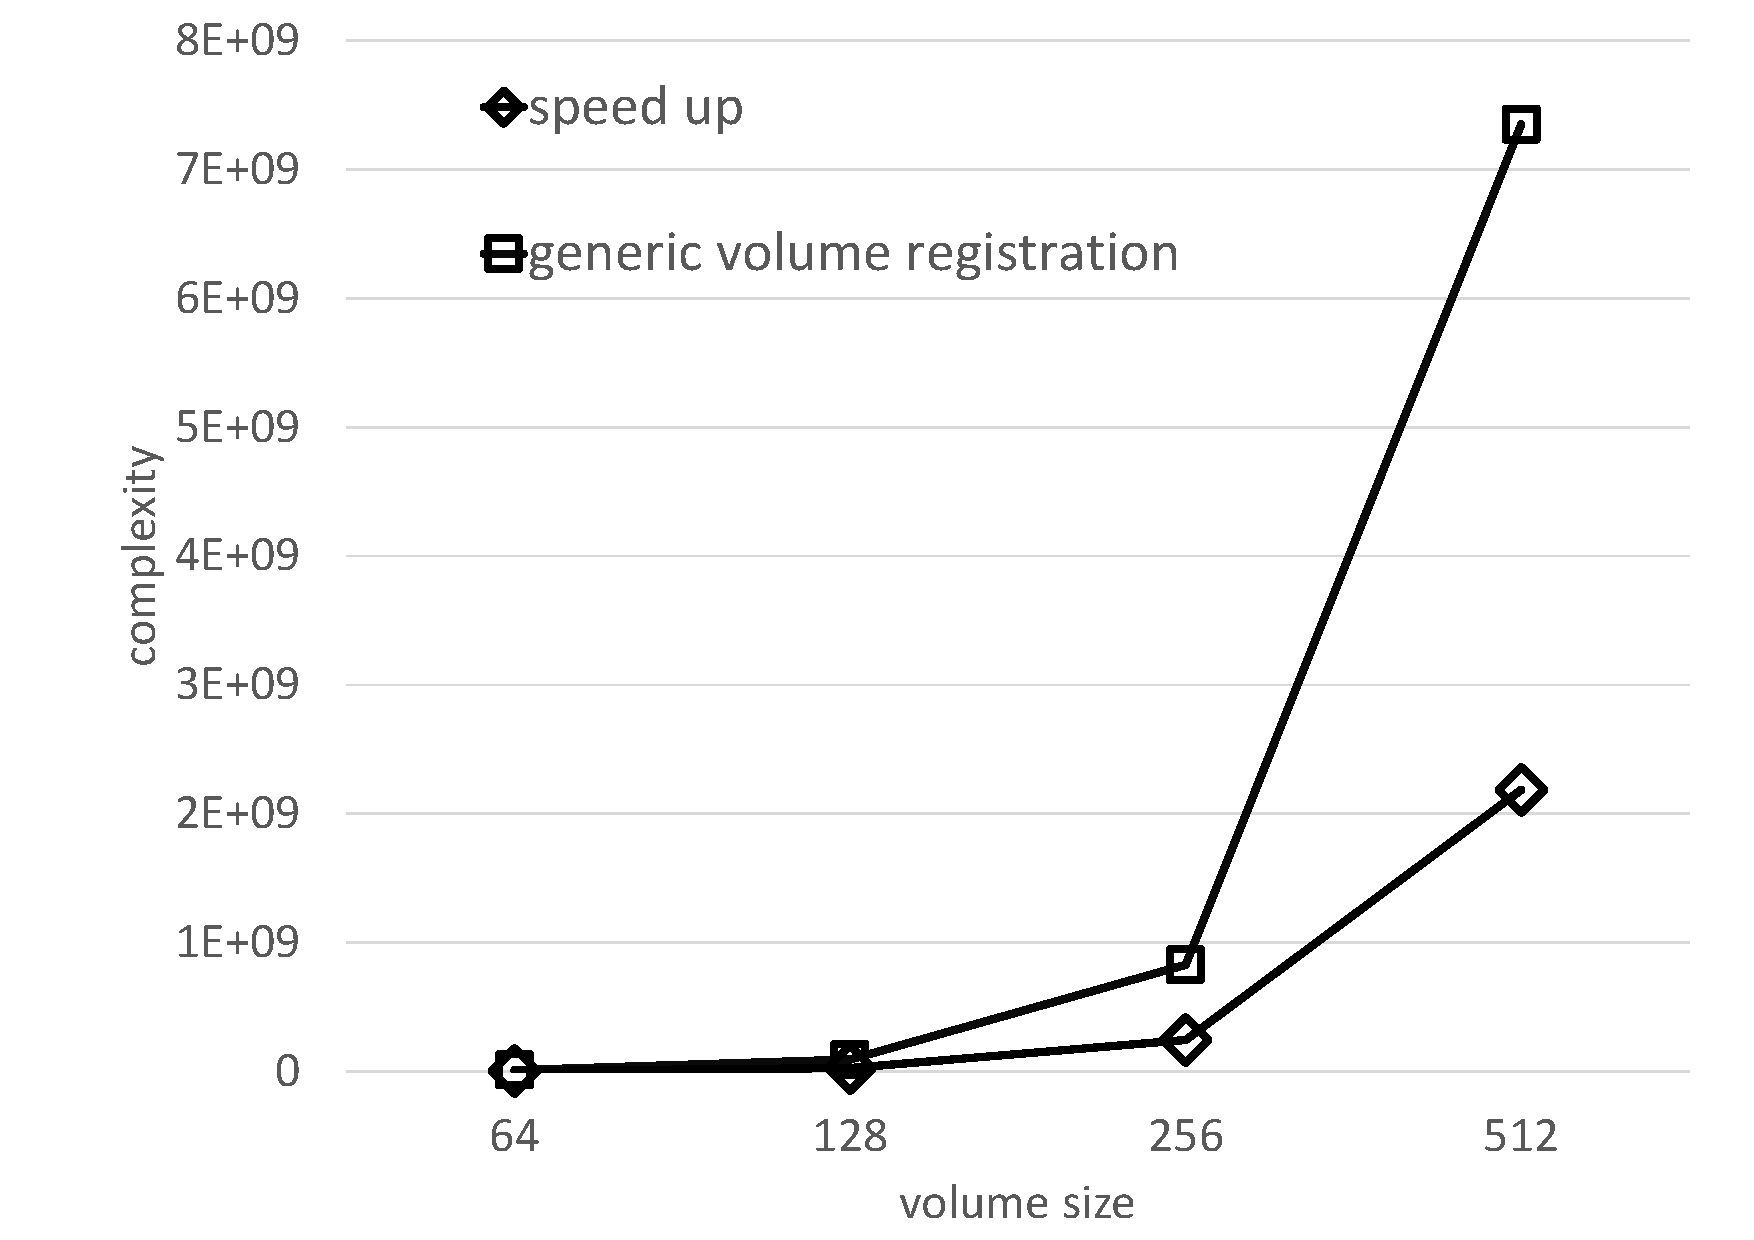
\includegraphics[width=4.0in]{images/ch2/perfcomp}
\caption{Comparison of performance between volume registration and the proposed speed up for different volume sizes.}
\label{fig:perfComp}
\end{figure}

